\documentclass[Serif, 10pt, brown]{beamer}
\usepackage{booktabs,xcolor}
%\usepackage[svgnames,table]{xcolor}
%\usepackage[tableposition=above]{caption}
\usepackage{pifont}
\newcommand*\CHECK{\ding{51}}
\usepackage{array}
\newcolumntype{P}[1]{>{\centering\arraybackslash}p{#1}}
%
\usepackage{setspace,mathtools,amssymb,multirow,array,amsmath,tikz}
\usepackage[normalsize]{subfigure}
\usetikzlibrary{patterns}
\usetikzlibrary{automata,positioning,decorations.pathreplacing,decorations}

\usepackage{curves}
\usepackage{wasysym}
\usepackage{epsfig,epstopdf,graphicx}

\curvewarnfalse
%
\newtheorem{proposition}{Proposition}
\theoremstyle{example}
\newtheorem{theoremh}{Theorem}
\theoremstyle{plain}
\renewcommand{\textfraction}{0.01}
\renewcommand{\floatpagefraction}{0.99}
\newcommand{\ul}{\underline}
\newcounter{units}
%
%
\setbeamercovered{dynamic}
% Logo
\logo{
\includegraphics[width=0.5in,keepaspectratio]{iitb_logo.png}}
%
% Setup
\mode<presentation>
	{
\usetheme[right,currentsection, hideothersubsections]{UTD}
			\useoutertheme{sidebar} \useinnertheme[shadow]{rounded}
			\usecolortheme{whale} \usecolortheme{orchid}
			\usefonttheme[onlymath]{serif}
			\setbeamertemplate{footline}{\centerline{Slide \insertframenumber/\inserttotalframenumber}}
	}
%
% Title
\usebeamercolor[fg]{author in sidebar}
\title[{CS349 Project}]{\sc Automatic Index Creation}
\author[\ul{Authors}]{{\bf { Saksham Rathi, Kavya Gupta, Shravan S, Mayank Kumar}}\\ {\footnotesize \hspace{0cm} (22B1003) \hspace{1cm} (22B1053) \hspace{0.5cm} (22B1054) \hspace{0.5cm} (22B0933)}}
\institute[UTD]{\sc\small CS349: DataBase and Information Systems\\ Under Prof. Sudarshan and Prof. Suraj}
\date[UCI]{Indian Institute of Technology Bombay \\ Spring 2024-25}
%
%Presentation
\begin{document}
\frame{\titlepage}
%
%
%Slides

%TOC

\begin{frame}
	\transblindsvertical
	\frametitle{Contents}
	\tableofcontents[hidesubsections]
\end{frame}

\section{Introduction}
\begin{frame}{Introduction to the Problem Statement}

	\begin{itemize}
		\item Indexes are crucial for efficient query execution in relational databases.
		\item However, developers sometimes forget to create indexes for frequently queried columns.
		\item This can lead to repeated full relation scans, significantly degrading performance.
		\item {\bf Goal:} Modify the application layer of PostgreSQL to detect such patterns and automatically create indexes when beneficial.
		\item Approach:
		\begin{itemize}
			\item Track full relation scans with equality predicates.
			\item Estimate the potential benefit of an index.
			\item Automatically trigger index creation if estimated benefit outweighs the cost.
			\item Rejecting low selectivity columns, such as gender, which has low number of distinct values.
		\end{itemize}
	\end{itemize}
\end{frame}

\section{Directory Structure}
\begin{frame}{Directory Structure}
	Here is the directory structure of the submission:
	\begin{itemize}
		\item \texttt{./code}: Contains the header and C++ files for the implementation, along with the Makefile.
		\item \texttt{./theory}: Contains some relevant paper and slides.
		\item \texttt{./documentation}: Contains the report as \texttt{readme.pdf}.
		\item \texttt{./README.md}: Contains the instructions to run the code.
	\end{itemize}
\end{frame}

\section{When to use indices?}
\begin{frame}{About Indices}
	An index in SQL is a database object that improves the speed of data retrieval operations on a database table. 

	\vspace{1cm}

	When a query is executed, the database can use the index to quickly find the relevant rows. 

	\vspace{1cm}

	Without an index, the database might need to scan every row to find the data, which is much slower.
\end{frame}

\begin{frame}{When to use indices?}
	\begin{itemize}
		\item {\bf Frequent searches on specific columns:} Columns that are often used in WHERE clauses, JOIN conditions or as part of a SELECT query.
		\item {\bf Large Tables with Heavy Read Operations:} Tables with a vast number of records where read operations are more common than write operations.
		\item {\bf Columns used in JOINs:} Indexing these columns can speed up the join process.
		\item {\bf Unique or Primary Key Constraints:} Indices improve lookup efficiency, so easy to impose such constraints.
		\item {\bf Composite Indices:} When queries often filter on multiple columns, a composite index can be beneficial, rather than creating separate indices for each column.
	\end{itemize}
\end{frame}

\begin{frame}{When to use indices?}
	There are also cases, where we should refrain from using indices, such as tables with heavy write operations, because indices slow down INSERT, UPDATE, and DELETE operations (index needs to be updated too). Similarly, in case of small tables, or columns with low selectivity (many duplicate values).

	\vspace{1cm}

	Indices, overall lead to improved query performance, slower write opterations, and increased storage requirements.
	
	\vspace{1cm}

	We can analyze how a query is execueted, and whether an index is effectively used or not by using the \texttt{EXPLAIN} command in PostgreSQL. Moreover, to maintain performance, expecially in databases with frequent data modifications, we need to regularly rebuild and reorganize indices.
\end{frame}

\section{An Auto-Indexing Technique for Databases Based on Clustering}

\begin{frame}{An Auto-Indexing Technique for Databases Based on Clustering}
	\begin{itemize}
		\item Automate the physical design so that the task of the database administrator (DBA) is minimized.
		\item The first category is external tools which use linear programming optimization techniques and other cost minimization techniques to solve the Index Selection Problem.
		\item The second category is the tools that utilize the query optimizer to give cost estimates for various index
		configurations and suggest a configuration with the least cost estimation.
		\item In this technique the optimizer is invoked only once for each query in the workload to choose the final set of indexes from a set of externally determined index configurations.
		\item All other details can be found in the next sections.
	\end{itemize}
\end{frame}

% \begin{frame}{Identifying Candidate Indexes}
% 	\begin{itemize}
% 		\item A query attribute matrix is created.
% 		\item The presence of an indexable attribute is created by 1 and absence by a 0.
% 		\item The condition applied is:
		
% 		\texttt{Freq > threshold1 OR Freq * T > threshold2}
% 		\item \texttt{Freq} is the frequency of each indexable attribute in the workload and \texttt{T} is proportional to the size of the table in rows to which the column belongs.
% 		\item Weights of 3, 2, 1 are given to the columns occurring in a {\tt WHERE} clause, {\tt GROUP BY} or {\tt ORDER BY} clauses and aggregate functions, respectively.
% 		\item During the clustering phase queries that are similar based on common and frequently occurring attributes are clustered together.
% 	\end{itemize}
% \end{frame}

% \begin{frame}{Candidate index suggestion}
% 	\begin{itemize}
% 		\item During this phase, those candidate indexable attributes which are common to all the queries clustered together during the clustering phase are suggested as indexes.
% 		\item The optimizer uses its statistics and cost estimates to choose indexes for each query.
% 		\item Those indexes not being picked up by the optimizer are dropped because the presence of these unused indexes will cause an overhead of space and maintenance in the database.
% 	\end{itemize}
% \end{frame}


\section{Goals}
\begin{frame}{Goals of the project}
	\begin{itemize}
		\item Indexes are crucial for efficient query execution in relational databases.
		\item However, developers sometimes forget to create indexes for frequently queried columns.
		\item This can lead to repeated full relation scans, significantly degrading performance.
		\item {\bf Goal:} Modify the application layer of PostgreSQL to detect such patterns and automatically create indexes when beneficial \cite{nagesh2023indexes}.
		\item {\bf Another Goal} was to understand and implement the paper \textit{``An Auto-Indexing Technique for Databases Based on Clustering''} \cite{1333569}.
	\end{itemize}
\end{frame}

\section{What We Implemented From User Perspective}
\begin{frame}{What We Implemented From User Perspective}
	\begin{itemize}
		\item We implemented an interface that can take and submit queries from users as usual as well as automatically create (and remove) indices appropriately, thereby improving performance without any user intervention.
	\end{itemize}
\end{frame}

\section{What All Functionalities We Implemented}
\begin{frame}{What All Functionalities We Implemented}
	\begin{itemize}
		\item Developed a standalone C++ tool that takes SQL queries as input and performs real-time analysis.
		\item Implemented policy from the paper \textit{``An Auto-Indexing Technique for Databases Based on Clustering''} \cite{1333569}.
		\item The tool tracks attribute access frequencies and cost, and forks a background process to decide on index creation.
		\item Index creation is not based on fixed thresholds alone:
		\begin{itemize}
			\item It also invokes the PostgreSQL query planner to compare costs of executing the current query for different candidate indices.
			\item Index is created only if the cost savings are significant.
		\end{itemize}
		\item Also integrated removal of indices using 2 policies:
	\end{itemize}
\end{frame}

\section{How We Implemented It}
\begin{frame}{How We Implemented It – Part 1}
	\begin{itemize}
		\item Used the \texttt{pqxx} C++ library to connect and interact with PostgreSQL databases.
		\item Integrated the \texttt{sqlparse} Python library to parse complex SQL queries and extract attribute-level access details.
		\item Designed custom data structures to:
		\begin{itemize}
			\item Maintain per-query attribute access statistics.
			\item Track information about the existing (our tool made) indices.
		\end{itemize}
		\item Queries are handled online (i.e., one at a time), so query clustering was not required, unlike in batch-based approaches.
	\end{itemize}
\end{frame}

\begin{frame}{How We Implemented It – Part 2}
	\begin{itemize}
		\item \textbf{Candidate attribute selection} is based on the following condition:
		\vspace{-5pt}
		\[
		\texttt{Freq} > \texttt{threshold}_1 \quad \textbf{OR} \quad \texttt{Freq} \times T > \texttt{threshold}_2
		\vspace{-5pt}
		\]
		where:
		\begin{itemize}
			\item \texttt{Freq} = weighted frequency of attribute usage in past queries.
			\item \texttt{T} = number of rows in the table containing that attribute.
		\end{itemize}
		We fixed $\texttt{threshold}_1$ to be $10$. We took $\texttt{threshold}_2$ as the average of the size of all tables in the database (we change it every $50^{th}$ iteration).
	
		\item \textbf{Weighted frequency computation}:
		\begin{itemize}
			\item Weight = 3 if attribute is in \texttt{WHERE} clause.
			\item Weight = 2 if in \texttt{GROUP BY} or \texttt{ORDER BY}.
			\item Weight = 1 if used in an aggregate function (e.g., \texttt{SUM}, \texttt{COUNT}).
		\end{itemize}
		This helps prioritize attributes more critical to query performance.
	\end{itemize}
\end{frame}

\begin{frame}{How We Implemented It – Part 3}
	\begin{itemize}
		\item Once candidate indexable attributes are identified (via frequency and weights), we use the \textbf{\texttt{hypopg}} extension for final selection.
		
		\item \texttt{hypopg} allows us to:
		\begin{itemize}
			\item Create \textbf{hypothetical indexes} without modifying the database.
			\item Run the SQL query planner with these indexes as if they existed.
			\item Retrieve the estimated query execution cost from the planner.
		\end{itemize}
	
		\item This approach enables us to:
		\begin{itemize}
			\item Leverage PostgreSQL’s internal \textbf{statistics and heuristics}.
			\item Avoid wasting resources on ineffective indexes.
		\end{itemize}
	
		\item The top 50\% lowest cost of the candidate indices become the final indices and index is created for them in a child process (if not already).
	\end{itemize}
\end{frame}

% \begin{frame}{How We Implemented It - Index Eviction}
% 	We have implemented two policies for index eviction:
% 	\begin{itemize}
% 		\item 
% 	\end{itemize}
	
% \end{frame}

\begin{frame}{How We Implemented It - Index Eviction}
    We have implemented two policies for index eviction:
    \begin{itemize}
        \item \textbf{Policy P1: Time-based Eviction} \\
        Indices that are older than a threshold (5 discrete events) are removed from the list and dropped from the database. This ensures that short-lived, potentially less useful indices are cleaned up promptly.

        \item \textbf{Policy P2: Usage-based Eviction} \\
        Indices are evicted if their age (current\_timestamp - create\_time) is more than four times the number of accesses. This removes infrequently used indices that have become stale, balancing age and usage.
    \end{itemize}
\end{frame}


\section{Results}
\begin{frame}{Results}
	\begin{figure}
        \centering
        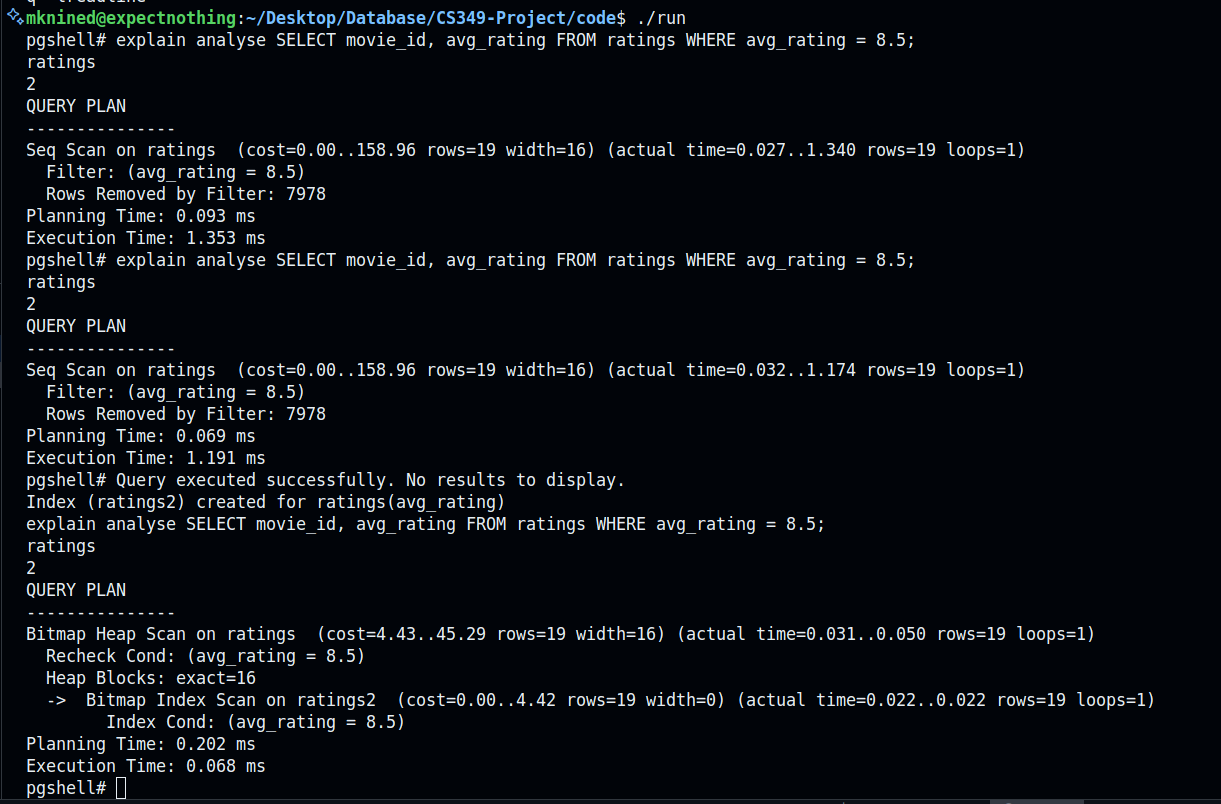
\includegraphics[width=1\linewidth]{../images/Screenshot from 2025-05-01 11-27-38.png}
        \caption{A sample run}
        % \label{fig:enter-label}
    \end{figure}
\end{frame}

\begin{frame}{Results}
	\begin{figure}
        \centering
        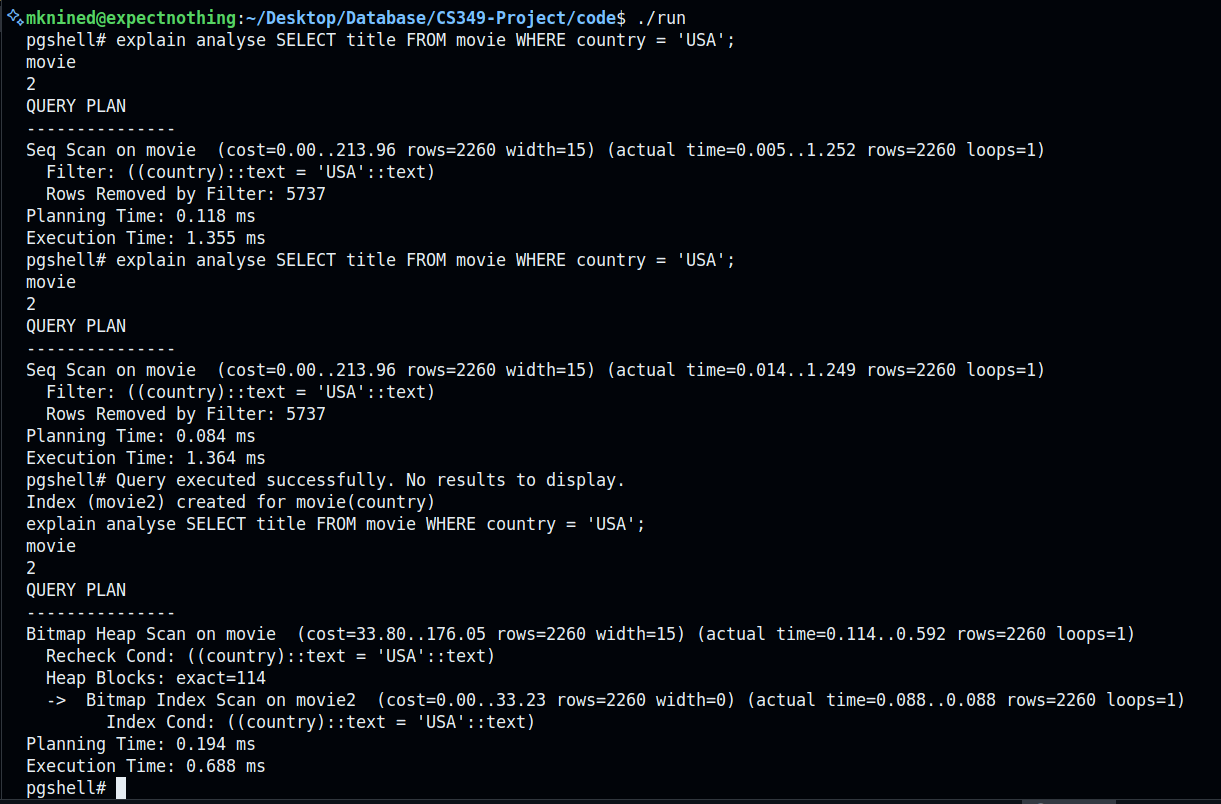
\includegraphics[width=1\linewidth]{../images/Screenshot from 2025-05-01 11-35-24.png}
        \caption{A sample run}
        % \label{fig:enter-label}
    \end{figure}
\end{frame}

\begin{frame}{Results}
	\begin{figure}
        \centering
        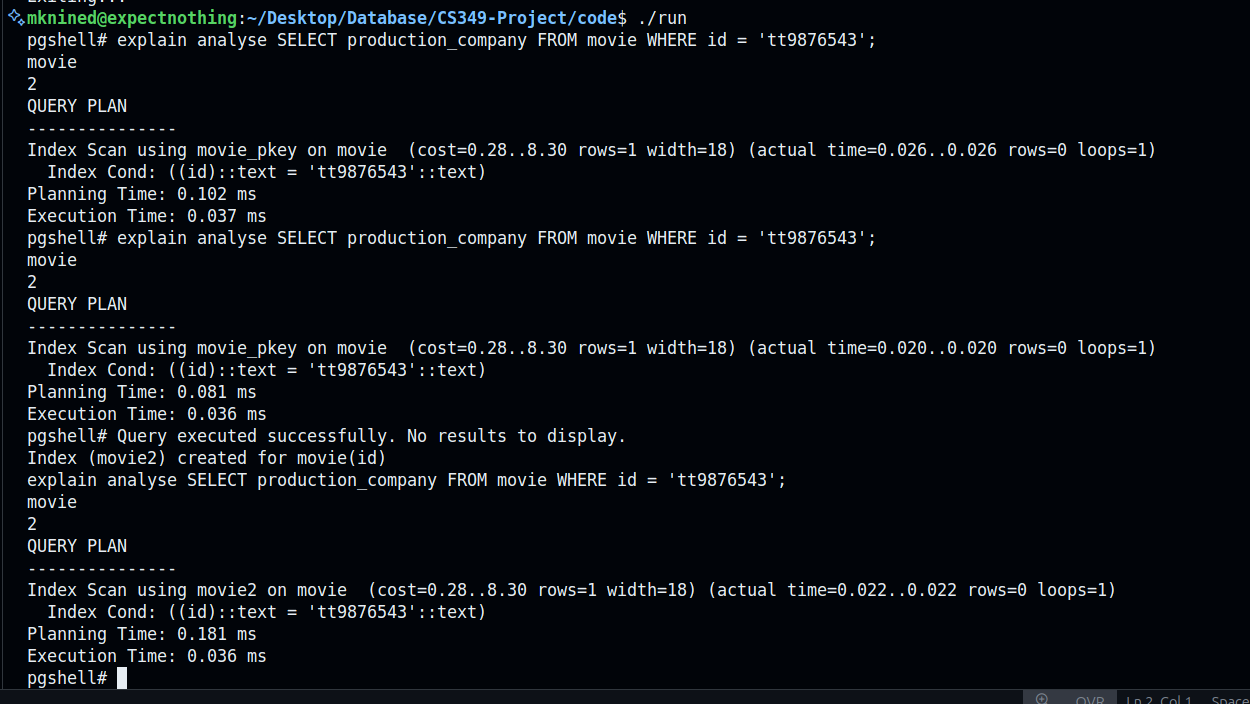
\includegraphics[width=1\linewidth]{../images/Screenshot from 2025-05-01 11-37-42.png}
        \caption{A sample run}
        % \label{fig:enter-label}
    \end{figure}
\end{frame}

\begin{frame}{Information about the Dataset}
	\begin{figure}
        \centering
        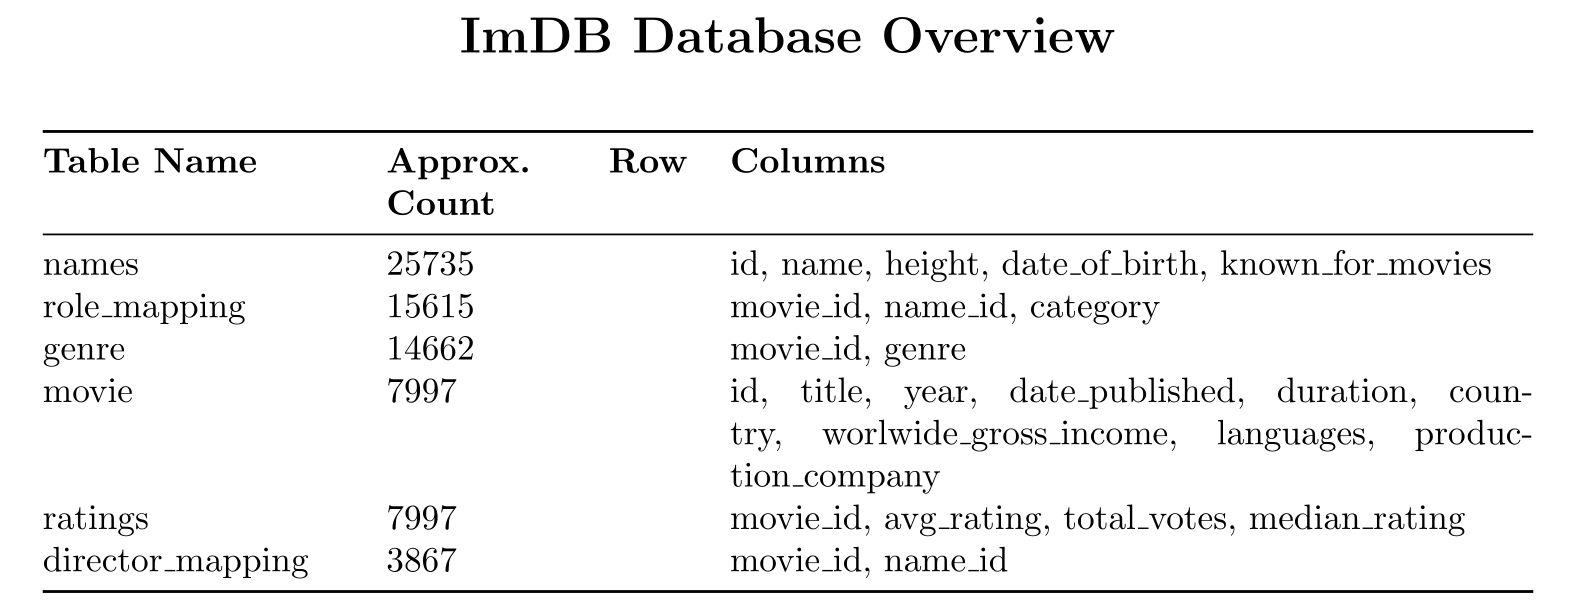
\includegraphics[width=1\linewidth]{../images/Screenshot from 2025-05-01 12-10-35.png}
        % \caption{A sample run}
        % \label{fig:enter-label}
    \end{figure}
\end{frame}
\section{Conclusion and Future Work}
\begin{frame}{Conclusion and Future Work}
	\begin{itemize}
		\item We developed a real-time auto-indexing system that:
		\begin{itemize}
			\item Tracks attribute access patterns and frequencies.
			\item Applies a cost-aware filtering mechanism using PostgreSQL’s planner via \texttt{hypopg}.
			\item Automatically creates and removes indexes using adaptive policies.
		\end{itemize}
	
		\vspace{0.3cm}
		\item \textbf{Future Work:}
		\begin{itemize}
			\item Extend the system to handle batch workloads.
			\item Incorporate clustering of similar queries to identify shared indexable patterns.
			\item Explore reinforcement learning or predictive models for smarter index management.
			\item Enhance the parser for better weighing mechanisms.
		\end{itemize}
	\end{itemize}
	\end{frame}

\section{References}
\begin{frame}{References}
	\bibliographystyle{alpha}
    \bibliography{ref}
\end{frame}

\begin{frame}{Code and Report}
    The code and the report can be found at the following link:
    \begin{center}
        \url{https://github.com/sakshamrathi21/CS349-Project}
    \end{center}
\end{frame}

\begin{frame}
    \Huge{\centerline{\bf Thank You}}
\end{frame}

\end{document}


